% Straight up stealing preamble from Eli Holmes 
%%%%%%%%%%%%%%%%%%%%%%%%%%%%%%%%%%%%%%START PREAMBLE THAT IS THE SAME FOR ALL EXAMPLES
\documentclass{article}

%Required: You must have these
\usepackage{Sweave}
\usepackage{graphicx}
\usepackage{tabularx}
\usepackage{hyperref}
\usepackage{natbib}
\usepackage{pdflscape}
\usepackage{array}
\usepackage{gensymb}
%\usepackage[backend=bibtex]{biblatex}
%Strongly recommended
  %put your figures in one place
%\SweaveOpts{prefix.string=figures/, eps=FALSE} 
%you'll want these for pretty captioning
\usepackage[small]{caption}

\setkeys{Gin}{width=0.8\textwidth}  %make the figs 50 perc textwidth
\setlength{\captionmargin}{30pt}
\setlength{\abovecaptionskip}{10pt}
\setlength{\belowcaptionskip}{10pt}
% manual for caption  http://www.dd.chalmers.se/latex/Docs/PDF/caption.pdf

%Optional: I like to muck with my margins and spacing in ways that LaTeX frowns on
%Here's how to do that
 \topmargin -1.5cm        
 \oddsidemargin -0.04cm   
 \evensidemargin -0.04cm  % same as oddsidemargin but for left-hand pages
 \textwidth 16.59cm
 \textheight 21.94cm 
 %\pagestyle{empty}       % Uncomment if don't want page numbers
 \parskip 7.2pt           % sets spacing between paragraphs
 %\renewcommand{\baselinestretch}{1.5} 	% Uncomment for 1.5 spacing between lines
\parindent 0pt% sets leading space for paragraphs
\usepackage{setspace}
%\doublespacing

%Optional: I like fancy headers
%\usepackage{fancyhdr}
%\pagestyle{fancy}
%\fancyhead[LO]{How do climate change experiments actually change climate}
%\fancyhead[RO]{2016}
 
%%%%%%%%%%%%%%%%%%%%%%%%%%%%%%%%%%%%%%END PREAMBLE THAT IS THE SAME FOR ALL EXAMPLES

%Start of the document
\begin{document}

%\SweaveOpts{concordance=TRUE}
 \bibliographystyle{/Users/aileneettinger/citations/Bibtex/styles/amnat.bst}
\title{Spatial and temporal shifts in photoperiod with climate change} % perspective paper for OSPREE analyses

\author{A.K. Ettinger, D. Buonaiuto, C. Chamberlain, I. Morales-Castilla, E. Wolkovich}
%\date{\today}%do we need to also add any of the following: D. Flynn, T. Savas, J. Samaha, E. Forrestel? 
\maketitle  %put the fancy title on
%\tableofcontents      %add a table of contents
%\clearpage
%%%%%%%%%%%%%%%%%%%%%%%%%%%%%%%%%%%%%%%%%%%%%%%%%%%

%%%%%%%%%%%%%%%%%%%%%%%%%%%%%%%%%%%%%%%%%%%%%%%%%%%

\section*{Summary}
Recent warming temperatures have brought about temporal shifts in biological activity, such as spring budburst, as well as spatial shifts in species' distributions. Both temporal and spatial shifts are expected to continue with future warming, and will alter the photoperiod experienced by diverse species. To date, photoperiod has not been a focus of climate change forecasting, despite the fact that photoperiod responses are common (observed in 26/31 or 84\% of studies that manipulated photoperiod in woody plant species). We argue that temporal shifts are expected to have a major impact on experienced photoperiod. Thus, improving our mechanistic understanding of the role of photoperiod in spring phenology and incorporating photoperiod into forecasts of biological shifts should be major goals. % Fierdre says: the previous 2 sentences are passive and could benefit from stronger wording.
We find that there already exists a substantial resource of growth chamber experiments with relevant treatments that could be used to forecast implications of photoperiod shifts with climate change. We highlight outstanding questions that are in need of additional research and modelling approaches to improve predictions of when, where, and how much photoperiod is likely to affect future spring phenology.

\section*{Introduction}
\par Shifts in the timing of spring events --- including flowering, bird arrival, egg hatching and myriad other activities --- are some of the most widely documented biological signals of climate change. Across taxa from plants and insects to mollusks and mammals, spring phenology is occurring earlier as temperatures warm, with average shifts of 1.2 to 5.1 days earlier per decade \citep{bradley1999,parmesan2003, root2003} or 1.3 to 5.6 days earlier per \degree C of warming\citep{wolkovich2012,polgar2013}. Indeed, early spring phenology appears to be shifting more rapidly than later season phenology in many cases \citep{bradley1999,menzel2006}, suggesting strong temperature sensitivity of spring phenophases.

\par Spring phenology is not controlled solely by temperature, however. Photoperiod is also a critical cue for plants and animals, signalling changes in growth, mating, and reproduction across diverse species \citep[e.g.,][]{Howe:1996,flynn2018,solbakken1994,mcallan2006,lagercrantz2009}. Photoperiod is used to synchronize activities with seasonal climatic changes \citep[e.g.,][]{Hsu:2011,Singh:2017,Basler:2012} because it is consistent across years, especially compared to other seasonal cues such as temperature and precipitation \citep{saikkonen2012}. For example, relying on photoperiod, rather than temperature alone, may prevent woody plants from leafing out during ``false spring" events \citep[unusually warm periods during winter that are followed by a return of cold temperatures][] {Gu2008}. 

\par Recent studies offer inconsistent views about whether photoperiod may eventually restrict spring phenology in a warmer world. Some studies suggest that certain species will be unable to track climate warming, i.e., by leafing out earlier in the spring \citep{koerner2010b,way2015}. Instead, these species will increasingly become constrained by daylength, since photoperiod sensitivity is primarily genetically controlled \citep{bradshaw2008}. Other studies, however, suggest that photoperiod is unlikely to constrain responses to warming for most species \citep{zohner2016,chuine2010}.

\par Interactions between temperature and photoperiod have been particularly well studied in woody plant phenology. Decades of experimental growth chamber studies have shown that photoperiod is an important cue for spring budburst phenology in woody plants. These experiments often manipulate photoperiod in combination with temperature to address basic questions about how these two environmental drivers act as biological cues. Air temperature has a dual role in regulating phenology: chilling, the prolonged exposure to cold temperatures after growth cessation in the fall, is required to initiate budburst; and forcing, prolonged exposure to warm temperatures, is required for budburst to occur. Thus, chilling and forcing treatments are often altered in addition to photoperiod in growth chamber experiments \citep[e.g.,][]{Campbell:1975aa,HEIDE:1977aa,Falusi:1990aa,Spann:2004aa,Laube:2014a}. Growth chamber studies have been conducted for decades, but have only recently been synthesized (cite main ospree bb paper), revealing wide variation in sensitivity to photoperiod across studies. 

\par Perhaps because of these variable responses across both experimental and observational studies, photoperiod is often not included in forecasts of biological responses to climate change even though it is known to be an important cue for plant activity \citet[but see ][]{duputie2015}. %%Diedre: It is not 100% clear to me that both trends were found in both experimental and observational studies. I only took away from the above paragraph that photoperiod was found to be important, not that its importance varied. % IMC- I'm not sure forecasts of biological responses to climate change focus on temperature. Most literature on SDMs forecasting species distributions uses a bunch of environmental variables (see http://worldclim.org/bioclim) to fit the models with subsequent problems of collinearity (but that's another topic). Perhaps we could mention, that amongst the 'usual suspect' environmental variables used to fit forecasts, photoperiod is rarely included.
The exclusion of photoperiod may be problematic because, although photoperiod itself is stable over time, the photoperiod that species \emph{experience}, as they undergo climate change-induced shifts in space and time, is likely to be much less stable. With recent warming, many species have shifted their distributions poleward and upward in elevation \citep[i.e., range shifts][]{parmesan2006,chen2011,harsch2009})), and/or shifted their activity earlier in the year \citep[i.e., phenological shifts][]{parmesan2006, wolkovich2012}. These spatial and temporal shifts will alter the photoperiod regime experienced by organisms (Figure \ref{fig:spacetime}). 

\par The implications of potential climate-change induced shifts in experienced photoperiod are unclear, since the magnitude of potential shifts has not been described. Shifts may be relatively minor, especially because there can be substantial year-to-year background variation in experienced photoperiod (Figure \ref{fig:greenup}). Alternatively, photoperiod may begin to constrain species responses to climate change \citep{koerner2010b}.

% IMC: I would include a citation to Pe?uelas' study on altitudinal shifts:
% @article{penuelas2003global,
%  title={A global change-induced biome shift in the Montseny mountains (NE Spain)},
%  author={Pe{\~n}uelas, Josep and Boada, Mart{\'\i}},
%  journal={Global change biology},
%  volume={9},
%  number={2},
%  pages={131--140},
%  year={2003},
%  publisher={Wiley Online Library}
%}....

\par Here, we ask: 
\begin{enumerate}
\item How will climate change alter the photoperiod experienced by organisms? %DB Im wondering if we should switch order of Q1 and 2. Q2 seems more like basic science and Q1 feels more similar to 3 and 4 with its direct applications to climate change.
\item Are photoperiod responses widespread in woody plants? %DB regardless of decision about above, perhaps we should justify this question more in the introduction. You say below: "the importance of photoperiod versus temperature effects on phenology remain controversial in woody species" but maybe adding a sentence to the paragraph "Recent studies...(line 73) that say more explicity something like "this unknown may stem for the the fact that photoperiod responses seems to be inconsistant across taxa, and there is no consensis about how common, or strong the photoperiod response is across woody plants". CJC: I agree with Dan about switching around. You could also tack more onto the paragraph with OSPREE talking about how our results suggest variation in photoperiod sensitivity. 
\item What are the implications of altered photoperiods for biological responses to climate change?
\item Can data from growth chamber experiments altering photoperiod be applied to forecasting biological implications of climate change?

\end{enumerate}
\par We address these questions using OSPREE, a new database of plant growth chamber studies that manipulate photoperiod and temperature and measure plant responses, including budburst, flowering, and growth (cite OSPREE database on knb?).          .  %The database includes studies that manipulate photoperiod by applying treatments with different daylength durations, applying long-day versus short-day conditions for different lengths of time, and/or applying varying vs contant photoperiods. 
We focus on woody species because plant growth chamber experiments using woody plant material have been conducted for decades, because the importance of photoperiod versus temperature effects on phenology remain controversial in woody species, and because forecasting effects of climate change on woody plant phenology (i.e., the length of the growing season) has critical implications for global carbon cycling and feedbacks to the climate system (add citations). 

\section*{How will climate change alter the photoperiod experienced by organisms?}
\par Species experience different photoperiod regimes depending on their location on Earth and the seasonal timing of their activity. The daylength experienced by plants on spring green-up date, for example, varies with latitude (Figure \ref{fig:greenup}a). This is in part because of latitudinal variation in green-up date, which occurs earlier toward the equator and later toward the north pole, likely driven by climatic differences, and in part because of latitudinal variation in photoperiod (e.g., at the north pole, the daylength at the summer solstice is 24 hours). A general pattern of longer photoperiod at green-up toward the poles is consistent across years (Figure \ref{fig:greenup}b) and green-up does not appear to occur at daylengths less than 10 hours. However, there is strong spatiotemporal variation in experienced photoperiod when differences across years (e.g., years with ``early" versus ``late" green-up) are considered. Experienced photoperiod at green-up can vary by as much as two to three hours in the same location (Figure \ref{fig:greenup}c).

\par Against this existing background variation, climate change is likely to cause average shifts in experienced photoperiod, as species respond to warming temperatures. Spatial shifts in species' ranges and temporal shifts in phenology will alter the photoperiods experienced by organisms with future climate change. The magnitude of these alterations will vary depending on the organism's location and the type of shift(s) it undergoes. For example, poleward shifts in species' ranges cause organisms to experience a wider range of daylength throughout the year (Figure \ref{fig:spacetime}). Elevational shifts, on the other hand, would cause minimal changes in the range of daylength throughout the year. %%IMC - do we have something to cite in support of this sentence? 
%AKE: I have not found a scientific publication yet- just back of the envelope calculations. for example, from https://www.chicagotribune.com/news/weather/ct-wea-0928-asktom-20160927-column.html: which states "Sunrise is one minute earlier for every 4,921.3 feet of height above sea level and one minute later for the same height. That is, two minutes of daylight are added for every 4,921.3 feet of altitude." 
\par To date, most of the scientific literature has focused on how spatial range shifts linked to climate change will affect photoperiod \citep[e.g.,] []{saikkonen2012, way2015}. Shifting phenology will also alter experienced photoperiod, because of the seasonal patterns of daylength (Figure \ref{fig:spacetime}). To understand the magnitude of change in experienced photoperiod with spatial versus temporal shifts in organisms' activities, we compared photoperiod across latitudes and dates that differed at relevant scales, given observed shifts in species' ranges and phenology \citep{parmesan2003,chen2011}.  
\par We found that temporal shifts are likely to yield much bigger changes in experienced photoperiod than spatial shifts (Figure \ref{fig:spacetime}). For example, consider a tree at latitude 45\degree  that completes spring budbursts, on average, around DOY 91 (April 2, when daylength is 12.8 hours). If its phenology shifts 30 days earlier over the next century \citep[][i.e., a rate of ~3 days per decade, as has been observed]{parmesan2003}, it will experience a daylength that is 1.6 hours shorter. However, if the same tree species shifts its range up in latitude 0.5\degree (i.e., 60 km over the next century,  comparable to observed rates \citep{parmesan2003, chen2011}), it will experience a daylength that differs by less than a minute on the same DOY. Growth chamber studies demonstrate that the magnitudes of daylength shifts we can expect with climate change (i.e., 1-2 hours of difference in daylength with temporal shifts over the next century) are substantial enough to affect spring phenology (Table \ref{table:phototreats}).  
\par In many cases organisms may shift both their geographic ranges and their phenology simultaneously. In addition, photoperiod sensitivity, or the degree to which phenology is controlled by daylength, can vary with latitude \citep{Howe:1996,saikkonen2012,Partanen:2005aa,Vihera-Aarnio:2006aa,Caffarra:2011b,gauzere2017}, perhaps because of population-level differences in sensitivity. With future climate change, it is unclear how these complications will affect the photoperiod experienced by organisms and if these shifts in photoperiod will have important implications for biological responses. Part of this lack of clarity stems from the fact that phenology (e.g., the day of year that an plant bursts its buds) both affects and is affected by experienced photoperiod: climate change-induced shifts in phenology alter experienced photoperiod, which in turn affects phenology.


\section*{Are photoperiod responses common in woody plants?}
%DL: Every paragraph of this section essentially starts the same, could at least one be changed to sound less repetitive?
\par Growth chamber experiments suggest that photoperiod responses are common in woody plant species, and, typically, longer days result in earlier and more rapid budburst \citep [e.g., ][]{Caffarra:2011a}. Thirty-one of the 85 studies in the OSPREE database included two or more different photoperiod treatments. Of these, 26 (84\%) found significant photoperiod main effects or significant interactive effects with temperature (Table \ref{table:phototreats}). Main effects included responses such as growth \citep[e.g., higher growth rates with longer days ][]{Ashby:1962aa}, budset \citep[e.g., more rapid induction of budset with shorter days][]{Howe:1995aa}, and reproduction \citep[e.g., increased flowering with longer days ][]{Heide:2012aa}. 
\par Growth chamber experiments highlight that responses to photoperiod vary depending on temperature conditions. For example, more rapid advancement of budburst was observed under long versus short days with low chilling, than with high chilling in \emph{Betula payrifera} \citep{Hawkins:2012} (Figure \ref{fig:photocurve}). Frequently, long photoperiods can compensate for low amounts of chilling during winter dormancy, resulting in enhanced cell growth \citep{Heide:1993,Myking:1995,Caffarra:2011b}.
\par Growth chamber experiments also demonstrate that, though photoperiod responses are common, they are variable (Figure \ref{fig:photocurve}). Responses to photoperiod differ by species \citep[e.g.,][]{Heide:1993a,Howe:1996,Basler:2012, Basler:2014aa,zohner2016,flynn2018}. % DL:Although I am a fan of short sentences, I found this one to just hang, could it be better integrated into the examples?
For example, with long chilling treatments some species seem insensitive to daylength (e.g.,Cat- could you add a sp or 2 from zohner), % They don't specify the species they just say that 112 (out of the 173 species they studied) did not respond to varying photoperiods with low chilling treatments and then with increased chilling treatments, even more species were insensitive to photoperiod.  Intermediate chilling, only 16 species responded to photoperiod and, with high chilling, only 4 species responded to photoperiod (i.e., Fagus crenata, F. orientalis, F. sylvatica, and Carya cordiformis). From the figures in the supplement, I can offer a few species that have "no photoperiod requirement" according the Zohner/Renner... Hammamelis vernalis, H. japonica, most Prunus species including P. serotina, P. padus, P. avium, Betula pendula, Alnus incana, Acer platanoides, A. campestre... to name a few! Photoperiod requirement really varies across Betula and Alnus. 
whereas others (e.g. \emph{Fagus} spp., Figure \ref{fig:fagus}A) seem to be highly sensitive to daylength, even with long chilling treatments \citep{zohner2016}. In addition, some species demonstrated an opposing response to photoperiod than typically observed: \emph{Tilia}, for example, showed delayed budburst with longer daylengths (Figure \ref{fig:photocurve},\citep{Ashby:1962aa}) %could also use heide93a for example: Long days reduced the thermal time to budburst in all flushing species except Sorbus acuparia and Rubus ideaus
Photoperiod sensitivity also varies by population and ecotype \citep[e.g.,][]{Partanen:2005aa,flynn2018} (Figure \ref{fig:photocurve}). For example, photoperiod effects on budburst were more significant for lower latitude populations of \emph{Betula pendula} and \emph{B. pubescens} \citep{Partanen:2005aa}. %% CJC: that's super interesting especially since Zohner dubbed B. pendula insensitive. 

\section*{What are the implications of altered photoperiods for biological responses to climate change?}
\par Clearly, daylength can play a role in controlling critical plant functions, including vegetative growth, cell elongation, budburst, and flowering \citep{Linkosalo:2006aa,erwin1998,sidaway2010, Hsu:2011,Heide:2011aa,Ashby:1962aa,Heide:2012aa,mimura2007}. Climate change-induced shifts in photoperiod are therefore likely to alter these functions. The direction and magnitude of such alterations will vary, however, because of variation in photoperiod sensitivity, and because photoperiod often interacts with other environmental drivers, such as temperature, to affect phenology. 

\par Over the past century, spring phenology has shifted earlier in diverse woody species \citep{menzel2000}, a pattern that, to date, can be largely explained by warming spring temperatures (i.e., increased forcing). Photoperiod may eventually become a limiting factor, however, constraining the ability of species to respond to additional warming \citep{koerner2010b,vitasse2013, Morin:2010aa,Nienstaedt:1966aa}. Interactions between photoperiod and temperature may therefore result in muted phenological shifts, compared to what would be expected based on temperature change alone \citep{wareing1956,mimura2007,koerner2010b}. If photoperiod does become limiting, the average trend of earlier phenology with warming may stop abruptly, because photoperiod sensitivity is thought to be a threshold response (Box 1). %define muted shifts? or explain more? or use a different word? was unclear to darwin

% 6 Dec 2018 (IMC): Not sure if this would make sense here, but we could talk about how the process of spatial-temporal shifts takes place by comparing populations of a species at the leading and trailing porgions of the range:
% If we think of a widely distributed species with e.g. 400km latitudinal range, equatorwards populations (trailing edge) will be experiencing stronger constraints by photoperiod, as warming will advance a lot the phenology, until reaching the photoperiod threshold below which survival is no longer possible.
% In poleward populations instead, although temperatures may be limiting, their interaction with increasing photoperiod may open an opportunity window for development.
% Obviously we don't need to expand on this, but maybe mention that the "detrimental/beneficial" effects of photoperiod*temperature interactions may differ across the range of a species.

\par A challenge in understanding biological responses to shifts in photoperiod is the wide range of sensitivity observed across species \citep{Sanz-Perez:2009aa, zohner2016,flynn2018}, populations \citep{tanino2010}, and ecotypes\citep{Howe:1995aa}. Some of this variation may be explained by different combinations of ambient temperature and photoperiod, because temperature cues can override photoperiod requirements under certain conditions \citep [at least during growth cessation][] {tanino2010}. In such cases, climate change induced phenological shifts may occur at different rates than past shifts with warming. However, a large portion of this variation is likely due to underlying genetic differences, because photoperiod responses are thought to be under strong genetic control \cite{bradshaw1995,weih2004,keller2011}. 
\par Species- and population-level variation in sensitivity to photoperiod may result in altered communities as climate change progresses. For example, a species or population that is relatively insensitive to photoperiod (or whose experienced photoperiod does not approach its critical photoperiod, even with climate change) will be able to take advantage of warmer springs by having an earlier start to its growing season. Such species (or populations) may therefore be able to outcompete slower growing ones that are limited by photoperiod and thus not able to take advantage of longer growing season conditions. In this way, sensitivity to photoperiod could act as a critical filter that alters plant communities with future climate change. 

% Also, do we know from OSPREE if small changes in photoperiod matter? CJC: I made a list of OSPREE papers for the latitue analysis that look at the effects of photoperiod. You can find it in /analyses/lat_analysis/photoperiodbylatitude_README.txt. Most found that photoperiod only really matters when not enough chilling and in some cases, when insufficient forcing. I did focus on latitude studies though so I may have missed other ones that strictly look at small photoperiod effects. 

\section*{Future directions: outstanding questions and incorporating photoperiod into forecasting}
\par  To identify where, when, and how plant communities may be altered, methods for incorporating photoperiod into forecasting future phenology will be critical. Incorporating photoperiod into forecasting is complex, since future rates of phenological shifts are unlikely be a straightforward extrapolation from current and past rates and because experienced photoperiod is both a driver and an effect of phenological shifts. Approaches for forecasts can be grouped into two broad categories: statistical models and process-based models. These two modelling extremes differ in at least two ways, in terms of relating plant phenology to climate change. First, statistical models generally assume linear relationships between species' responses and environmental variables \citep[e.g., OTHER EXAMPLES][]{flynn2018}, whereas process-based models incorporate nonlinear threshold relationships as well \citep[e.g.][]{chuine2001,morin2009}. Second, statistical models of phenology under climate change have typically ignored photoperiod, focusing instead on seasonal or annual temperature, % Or, as lizzie said: To date in statistical models many people either ignore photoperiod or they put it in in some very painful way ('we added photoperiod experienced on the day of budburst to the PEP725 data to test for the role of photoperiod') that is not well designed. 
whereas process-based models of phenology are more likely to incorporate photoperiod, along with forcing and chilling. The challenge of process-based models is that they require detailed data (e.g., daily climate data, nonlinear biological responses). Perhaps because of this challenge, statistical models remain more commonly used in climate change forecasts of biological responses \citep[e.g.,][]{Basler:2012}.%add some species distribution models that forecast
%DL: Is the challenge that this data is difficult to work with or hard/impossible to get? I think this point could be more explicit.
% 6 Dec 2018 IMC: Perhaps we should acknowledge some of the forestry literature using process-based models to forecast biological responses to climate change. I think the claim is true, but still, there is a lot of literature on forest process-based forecasts. We review some examples of this in Garc?a-Vald?s & Morales-Castilla (2016), but it is in Spanish so I'm not sure if you want to cite it. 
%   
\par Whether statistical or process-based approaches are used, future modelling can incorporate photoperiod by leveraging the large amount of experimental data on photoperiod responses (Figure \ref{fig:photomap}, Table \ref{table:phototreats}). Researchers can use these data to first learn if their species (or a closely related species) shows a photoperiod effect and, ideally, what its critical photoperiod is and how it varies by population, ecotype, or other factors. If there is evidence of a photoperiod response, daylength should be added to forecasting models, using the critical photoperiod to define short-day and long-day conditions (Figure \ref{fig:condiag}). Given the large change in experienced photoperiod with temporal shifts (Figure \ref{fig:spacetime}), this may be particularly important for phenology forecasting. Since spatial shifts are associated with smaller changes in experienced photoperiod, it may be less important for distribution forecasts.
That being said, species are likely to shift in \emph{both} space and time simultaneously. Thus, even though experienced photoperiod changes little as species distributions shift in space, phenology may be altered significantly, and have cascading effects on plant growth and fitness\citep{duputie2015}. 
\par For some species, experimental data can be immediately used in forecasting because experiments manipulate photoperiod at relevant scales (e.g., \citet{Basler:2014aa,Heide:2015aa}, Figures \ref{fig:photomap}, \ref{fig:fagus} A, Table \ref{table:phototreats}).  For example, photoperiod treatments from growth chamber experiments with \emph{Fagus sylvatica} span the variation in both current and expected future ranges (Figure \ref{fig:fagus}). In such cases, the available data can facilitate identifying critical photoperiod levels, and perhaps variations in critical photoperiod across populations (Figure \ref{fig:condiag}).  Adding photoperiod and variable responses to forecasts could fundamentally alter the future species and communities we expect, as discussed above. 

\par In other cases, attempting to incorporate photoperiod into forecasts of future phenology will highlight that there is a great need to better understand many aspects of photoperiod responses. For example, photoperiod treatments from  existing experiments of \emph{Quercus robur} do bracket the maxima and minima daylengths in current and expected future ranges (Figure \ref{fig:fagus}B). However, experimental datasets are missing many intermediate experienced photoperiods so finescale projections at many latitudes may be difficult. In these, and more extreme cases of species missing relevant data, modelling efforts may inspire additional experiments to test some of the critical predictions and assumptions that they make, and address outstanding questions in the field. Through the process of incorporating experimental data into more process-based models, it is likely that knowledge gaps will be identified. For example, many experiments manipulate photoperiod much more dramatically than will occur with climate change (Figures \ref{fig:photomap}, \ref{fig:fagus}). Although these studies are useful for understanding mechanistically how photoperiod responses work, extrapolating these findings to climate change models may be difficult. %DB cleaned up a few typos on March-7-2019
\par Additional areas of further research to improve our understanding of the effects of shifts in photoperiod with climate change include:
%change to paragraph form
\begin{enumerate}
\item \underline{How does photoperiod act as a cue?} The divergent effects of photoperiod observed across studies (e.g., Figure \ref{fig:photocurve}) suggests that photoperiod interacts with other environmental drivers, such as chilling and forcing, to affect phenology and other activities. However, exactly how it interacts with temperature to initiate budburst, as well as the type of response it elicits (e.g., linear versus threshold) and population- and species-specific critical photoperiods, are not well-defined for many species.  
\item \underline{Are there predictable mechanistic patterns in variation of photoperiod responses across species and populations? What are the consequences of this variation?} For example, what traits are associated with photoperiod sensitivity and does this variation have a strong genetic component? If so, are species or populations from some locations more likely than others to be constrained by photoperiod in their responses to climate change?

\item \underline{How inaccurate are current forecasts of biological responses to climate change, given that photoperiod \\ 
is not fully integrated?} Photoperiod is incorporated into forecasts, along with other variables such as evaporative demand, and temperature, in many ecosystem models \citep [e.g. ED] []{jolly2005, medvigy2013}, but is rarely included in species distribution models. The sensitivity of model outcomes to assumptions made about photoperiod, critical photoperiod, and photoperiod responses needs further study, for example, across ecosystems, species, and populations.

\end{enumerate}

\section*{Conclusions}
Organisms may undergo large changes to the photoperiod they experience, with climate change, even if they do not shift their ranges spatially.  Here, we have focused on how an altered photoperiod will affect woody plant budburst. Shifts in photoperiod with climate change are likely to have implications for a variety of plant and animal responses, given that daylength affects critical activities for diverse species from insects \citep{bradshaw2006,linn1996} and salmon \citep{solbakken1994,taranger2003} to birds \citep{dawson2001} and marsupials \citep{mcallan2006,solbakken1994}. Incorporating photoperiod into forecasting of climate change responses may improve model accuracy, and is likely to highlight additional experiments needed to improve our mechanistic understanding of photoperiod as a cue to diverse biological responses. 
\section* {Glossary}
\begin{itemize}
\item \underline{chilling}: the intensity and duration of winter temperature; critical chilling is the required amount of hours or days of cold temperature, defined by a specific critical temperature (e.g., 4 \degree C add citation), that must be experienced for budburst to occur.
\item \underline{daylength}: the period of time during a 24-hour period during which an organism receives light.
\item \underline{ecodormancy}: dormancy (e.g., halted or reduced growth) brought about by external conditions, such as cold temperatures or drought conditions. % CJC: maybe add something like "individuals can break dormancy during this time" whereas during endodormancy, individuals can't burst bud with a warm spell
\item \underline{endodormancy}: dormancy brought about by internal (rather than environmental) conditions. 
\item \underline{forcing}: warm spring temperatures, critical forcing is the required amount of hours or days above a specific temperature, that must be experienced before budburst or flowering can occur.
\item \underline{external coincidence model}: a model for how light sensing occurs in plants, first proposed by German biologist Erwin Bünning; it proposes the existence of a circadian rhythm of photoperiodic photosensitivity in which the night-phase is sensitive to light and the day-phase is insensitive to light. 
\item \underline{vernalization}: exposure of plants or seeds to low temperatures, often in order to stimulate flowering or to enhance seed production; analogous to chilling.
\item \underline{photoperiod}: the daily duration of light (daylength) and dark to which an organism is exposed; often used synonymously with daylength; critical photoperiod is the length of day that causes an individual to switch from a long-- to a short--day response (or vice versa).
\item \underline{photoperiodism}: the ability to assess the length of day or night to regulate behavior, physiology, growth, development or reproduction.
\end{itemize}
\section*{Box 1. Dominant models of how photoperiod affects spring phenology}
\par In this paper, we focus on spring budburst in woody plants, which is thought to be controlled by three main cues: chilling, forcing, and photoperiod, as well as interactions between them \citep{flynn2018,Heide:2008aa, zohner2016}. However, the molecular mechanisms and pathways underlying spring budburst are poorly understood \citep{ding2016}. Our understanding of how plants interpret photoperiod comes largely from studies of flowering in the model plant \emph{Arabidopsis thaliana} \citep[e.g.,][]{suarez2001} and budset in woody plant species \citep[e.g., ][]{Howe:1996}. Similar pathways may underlie budburst phenology in woody plants \citep{lagercrantz2009,ding2016}.
\par Plants sense light inputs by blue light receptors and phytochromes, which have been found in nearly all organs throughout the plant. Plants are thought to interpret photoperiod through a coordinated response to light in relation to the time of day. When the internal circadian rhythm coincides with an external signal (light) under certain conditions (e.g., warm days), a response is induced \citep{lagercrantz2009}. This ``external coincidence model" has been most widely studied in \emph{Arabidopsis}, and is thought to be a relevant mechanism for photoperiod responses in diverse perennial and woody plant species \citep{davis2002,petterle2013,bastow2002,kobayashi2007,andres2012,Singh:2017}. %add Bunning 1936).  
The model proposes the existence of a circadian rhythm of light sensitivity, in which the night-phase is sensitive to light and the day-phase is insensitive to light. As days get longer in the spring, daylight illuminates the  light sensitive phase, triggering a response. %DB do we want to show a schematic for this?
\par Little is known about the genetic pathways responsible for the light-sensing apparatuses involved in budburst, and how they may vary across species or populations. Some genes have been identified that play a role in coordinating budburst in poplar (\emph{Populus} spp.), and may occur in other woody species as well. Many similarities exist between the proposed regulatory networks of vegetative growth in \emph{Populus} and those controlling floral initiation in \emph{Arabidopsis}, \citet{ding2016}. For example, vegetative growth and inhibition of budset are promoted by the FLOWERING LOCUS T2 (FT2) gene, a homolog of \emph{Arabidopsis thaliana} gene FLOWERING LOCUS (FT). Promotion occurs in response to warm temperatures and long days, marking the onset of the growing season \citep{hsu2011}. FT2 expression appears to be controlled by a pathway that is effective in long days. Its loss of expression in autumn, when the days are getting shorter, is associated with the onset of dormancy \citep{glover2014}.
\par There are large gaps in our understanding of how photoperiod sensing pathways affect budburst, the genetics behind these pathways, and the extent of species- and population-level genetic variation. Questions also remain about how photoperiod sensing interacts with temperature sensing to affect responses. For example, Figure \ref{fig:photocurve} shows the most detailed data we were able to find of budburst responses across different photoperiod and chilling treatments. These data highlight how variable responses to photoperiod are, across species and populations, and with different chilling treatments. Additional growth chamber studies will be required to address the molecular mechanisms and genetic controls underlying this dramatic variation in  budburst responses to photoperiod. 

\section* {To do:}
\begin{enumerate}
\item incorporate comments from Lizzie, Cat, Dan, Nacho and Dierdre
\item Add more methods to supplement
\end{enumerate}

\bibliography{/Users/aileneettinger/Documents/GitHub/ospree/refs/ospreebibplus}
\clearpage


\section* {Tables}
% latex table generated in R 3.5.1 by xtable 1.8-3 package
% Tue Mar 26 09:34:19 2019
\begin{table}[ht]
\centering
\caption{\textbf{Growth chamber experiments and their photoperiod treatments}. We note whether or not photoperiod had a significant effect (`effect' column) and compared treatments to the spatial and temporal shifts required for organisms to experiments photoperiod changes equivalent to those treatments. For shifts in space, `ER' indicates that the photoperiod treatments exceeds the change of photoperiod from moving up to 40 degrees latitudinally on June 21. For shifts in time, `ER' indicates that the range of photoperiod treatments exceeds the change in daylengths at that latitude during the entire year. `max NA' indicates that the maximum daylength treatment does not exist at that latitude; `min NA'indicates that the minimum daylength treatment does not exist at that latitude.} 
\label{table:phototreats}
\begin{tabular}{|p{0.18\textwidth}|p{0.15\textwidth}|p{0.08\textwidth}|p{0.08\textwidth}|p{0.04\textwidth}|p{0.08\textwidth}|p{0.06\textwidth}|p{0.06\textwidth}|p{0.14\textwidth}|}
  \hline
idstudy & continent & lat & long & effect & day\_range & delta & space & time \\ 
  \hline
ashby62\_exp1 & north america & 42.99 & -89.41 & Y & 8-16 & 4.00 & 18.2 & -87* \\ 
  basler14\_exp1 & europe & 46.31 & 8.27 & Y & 9.2-16 & 1.00 & 6 & -22 \\ 
  caffarra11b\_exp2 & europe & 52.32 & -6.93 & Y & 10-16 & 2.00 & 7.5 & -30 \\ 
  falusi90\_exp1 & europe & 46.03 & 10.75 & N & 9-13 & 4.00 & 16 & -82 \\ 
  falusi96\_exp3 & europe & 38.27 & 15.99 & Y & 9-13 & 4.00 & 21.6 & -111 \\ 
  ghelardini10\_exp1 & europe & 43.72 & 11.37 & N & 8-16 & 8.00 & 21.9 & ER \\ 
  heide05\_exp1 & europe & 56.18 & -4.32 & Y/N & 10-24 & 14.00 & ER & ER \\ 
  heide08\_exp1 & europe & 48.40 & 11.72 & Y & 10-24 & 14.00 & ER & ER \\ 
  heide11\_exp1 & europe & 59.67 & 10.67 & N & 10-20 & 10.00 & ER & -117* \\ 
  heide12\_exp1 & europe & 56.50 & -3.06 & Y & 10-24 & 5.00 & 8.9 & -64 \\ 
  heide15\_exp2 & europe & 56.50 & -3.06 & Y & 10-15 & 1.00 & 3.2 & -13 \\ 
  heide93\_exp1 & europe & 59.50 & 10.77 & Y & 8-24 & 16.00 & ER & ER \\ 
  heide93a\_exp1 & europe & 59.67 & 10.83 & Y & 8-24 & 16.00 & ER & ER \\ 
  heide93a\_exp3 & europe & 47.50 & 7.60 & Y & 13-16 & 1.00 & 5.7 & -18 \\ 
  howe95\_exp1 & north america & 40.55 & -124.10 & Y & 9-24 & 2.00 & 13.1 & -64 \\ 
  laube14a\_exp1 & europe & 48.40 & 11.71 & N & 8-16 & 4.00 & 14.3 & -87 \\ 
  myking95\_exp1 & europe & 56.10 & 9.15 & Y & 8-24 & 16.00 & ER & ER \\ 
  nienstaedt66\_exp1 & north america & 44.17 & -103.92 & Y & 8-20 & 12.00 & ER & ER \\ 
  okie11\_exp1 & north america & 32.12 & -83.12 & Y & 0-12 & 12.00 & ER & ER \\ 
  partanen01\_exp1 & europe & 61.93 & 26.68 & Y & 6-16 & 10.00 & ER & -105 \\ 
  partanen05\_exp1 & europe & 61.82 & 29.32 & Y & 5-20 & 5.00 & ER & -67 \\ 
  partanen98\_exp1 & europe & 60.03 & 23.05 & Y & 8.66-12 & 3.34 & 5.1 & -37 \\ 
  pettersen71\_exp1 & europe & 59.66 & 10.77 & N & 10-24 & 2.00 & 4 & -23 \\ 
  Sanz-Perez09\_exp1 & europe & 40.40 & -3.48 & Y & 10-16 & 6.00 & 23.6 & ER \\ 
  viheraaarnio06\_exp1 & europe & 60.45 & 24.93 & Y & 16-17 & 1.00 & 2.1 & -12 \\ 
  viheraaarnio06\_exp1 & europe & 67.73 & 24.93 & Y & 20-21 & 1.00 & ER & -5 \\ 
  viheraaarnio06\_exp2 & europe & 60.45 & 24.93 & Y & 15-19 & 4.00 & 5.1 & -62 \\ 
  viheraaarnio06\_exp2 & europe & 67.73 & 24.93 & Y & 22-23 & 1.00 & ER & -3 \\ 
  worrall67\_exp 3 & north america & 41.31 & -72.93 & Y & 8-16 & 8.00 & 24.3 & ER \\ 
  zohner16\_Exp1 & europe & 48.16 & 11.50 & Y & 8-16 & 8.00 & ER & ER \\ 
  hawkins12\_ &  &  &  & Y &  &  &  &  \\ 
   \hline
\end{tabular}
\end{table}\clearpage
\section* {Figures}


\begin{figure}[p]
\centering
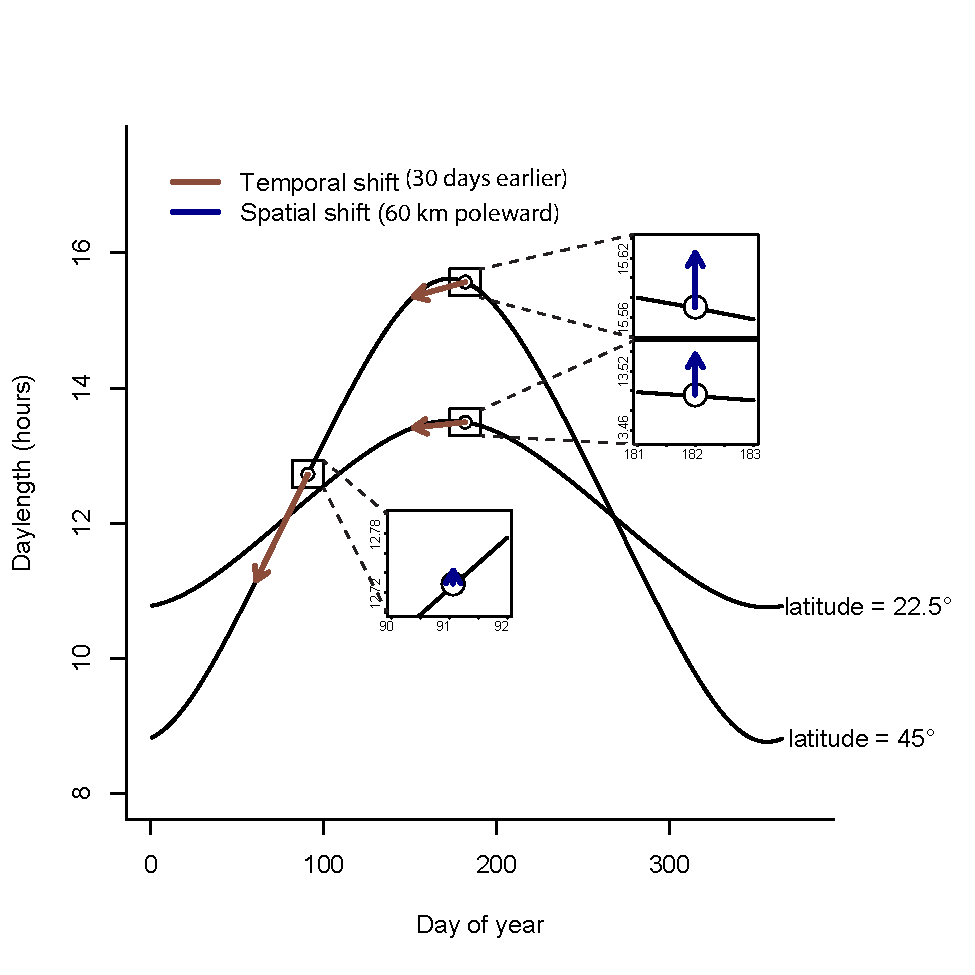
\includegraphics{/Users/aileneettinger/Documents/GitHub/ospree/analyses/photoperiod/figures/photo_spacetime_v2.pdf} %
\caption{\textbf{Photoperiod varies with latitude and throughout the year}, such that temporal shifts in activity yield larger changes in experienced photoperiod compared with spatial shifts. Here, we show this variation at two latitudes (22.5\degree, 45\degree), using hypothetical of spatial and temporal shifts. These shifts, which are similar to observed average rates with recent global warming \citep[e.g.,][]{parmesan2006,chen2011}, highlight the greater magnitude in daylength changes close to the equinox (e.g., DOY 91), versus close to the summer solstice (e.g., DOY 182).}
 \label{fig:spacetime}%
 \end{figure}
 
 \begin{figure}[p]
\centering
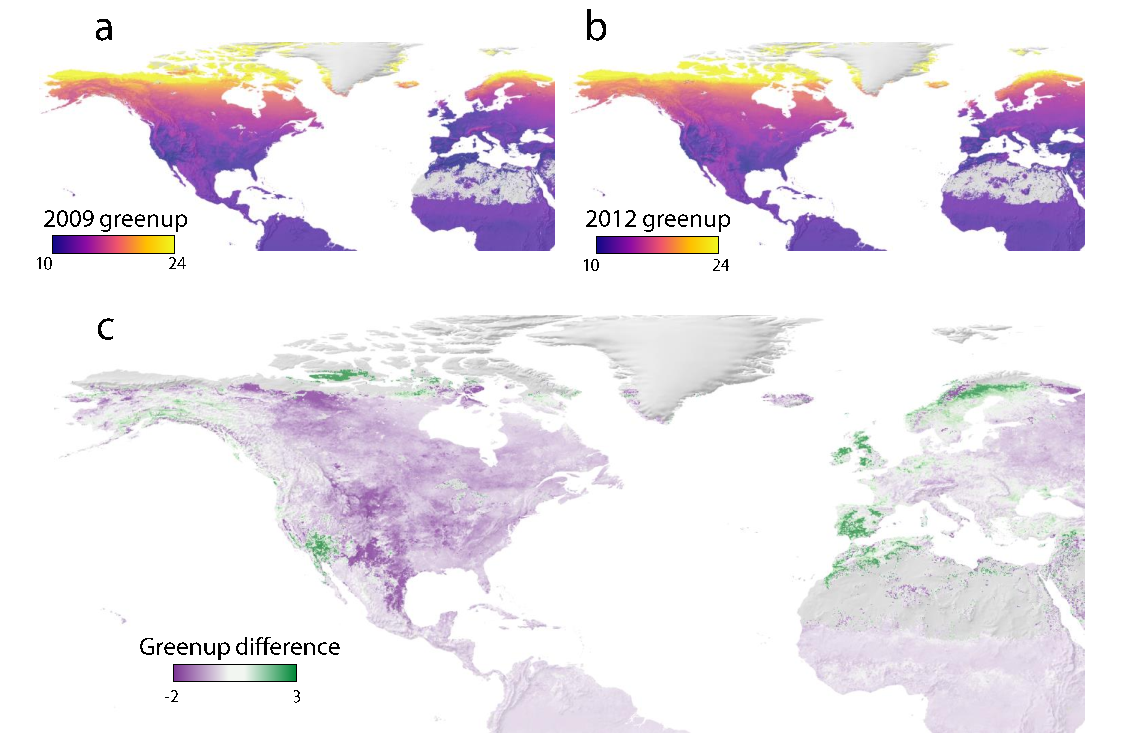
\includegraphics{/Users/aileneettinger/Documents/GitHub/ospree/docs/photoperiod/figures/Greenup_corr.pdf} %2009 greenup
\caption{\textbf{The photoperiod on the green up date (start of spring) varies over space} and among years. Hours of daylight on the date of spring green up from MODIS satellite data across North America and Europe for an average (2009, a) and  early (2012,b) North American start of spring. The differences between the years are shown in (c). }
 \label{fig:greenup}%
 \end{figure}
 
\begin{figure}[p]
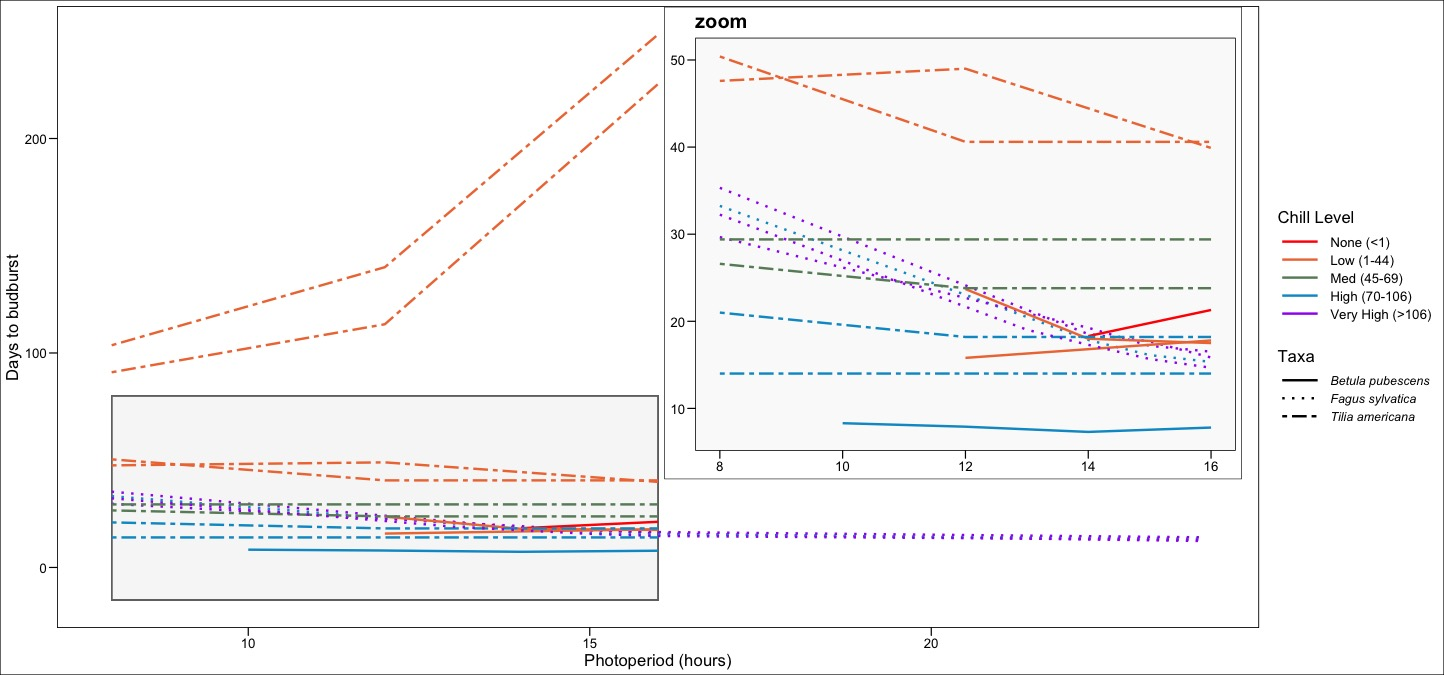
\includegraphics{/Users/aileneettinger/Documents/GitHub/ospree/analyses/photoperiod/figures/Photo_curv_FINAL.jpeg} 
\caption{\textbf{Nonlinearities in the phenological response to daylength} are apparent in experiments from the OSPREE database in which three or more photoperiod treatment levels were applied. The shape of the response curves for \textit{Betula pubescens} \citep{Caffarra:2011b}, \textit{Fagus sylvatica} \citep{Heide:1993a} and \textit{Tilia americana} \citep{Ashby:1962aa} differ depending on the amount of chilling recieved (in Chill portions). Species and chilling levels with multiple lines represent plant material from different populations.}
%Note: Hard to tell differene between Tilia and FAgus
 \label{fig:photocurve}
 \end{figure}


\begin{figure}[p]
\centering
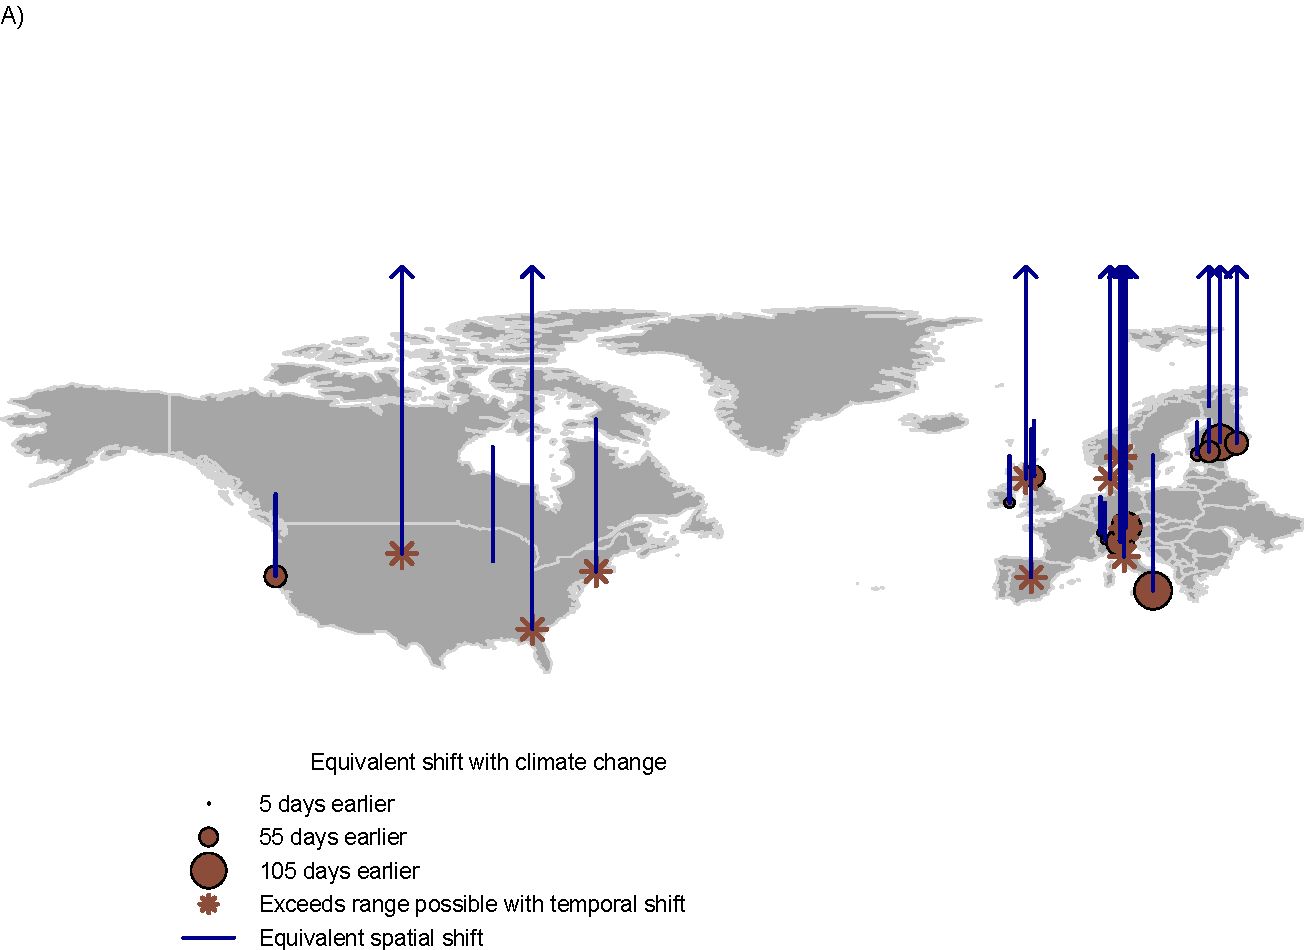
\includegraphics{/Users/aileneettinger/Documents/GitHub/ospree/analyses/photoperiod/figures/ospree_photopmap.pdf} 
\caption{\textbf{OSPREE experiments that manipulate photoperiod}, and their equivalent spatial and temporal shifts, mapped (A), and graphed (B-C). Observed rates (dashed gray lines) 16.9 kilometers per decade (or approximately 1.5 degrees in 100 years) for spatial shifts (Chen et al. 2011) and 2.3 days per decade (or 23 days in 100 years) for temporal shifts (Parmesan and Yohe 2003).}
 \label{fig:photomap}
 \end{figure}


 
 
\begin{figure}[p]
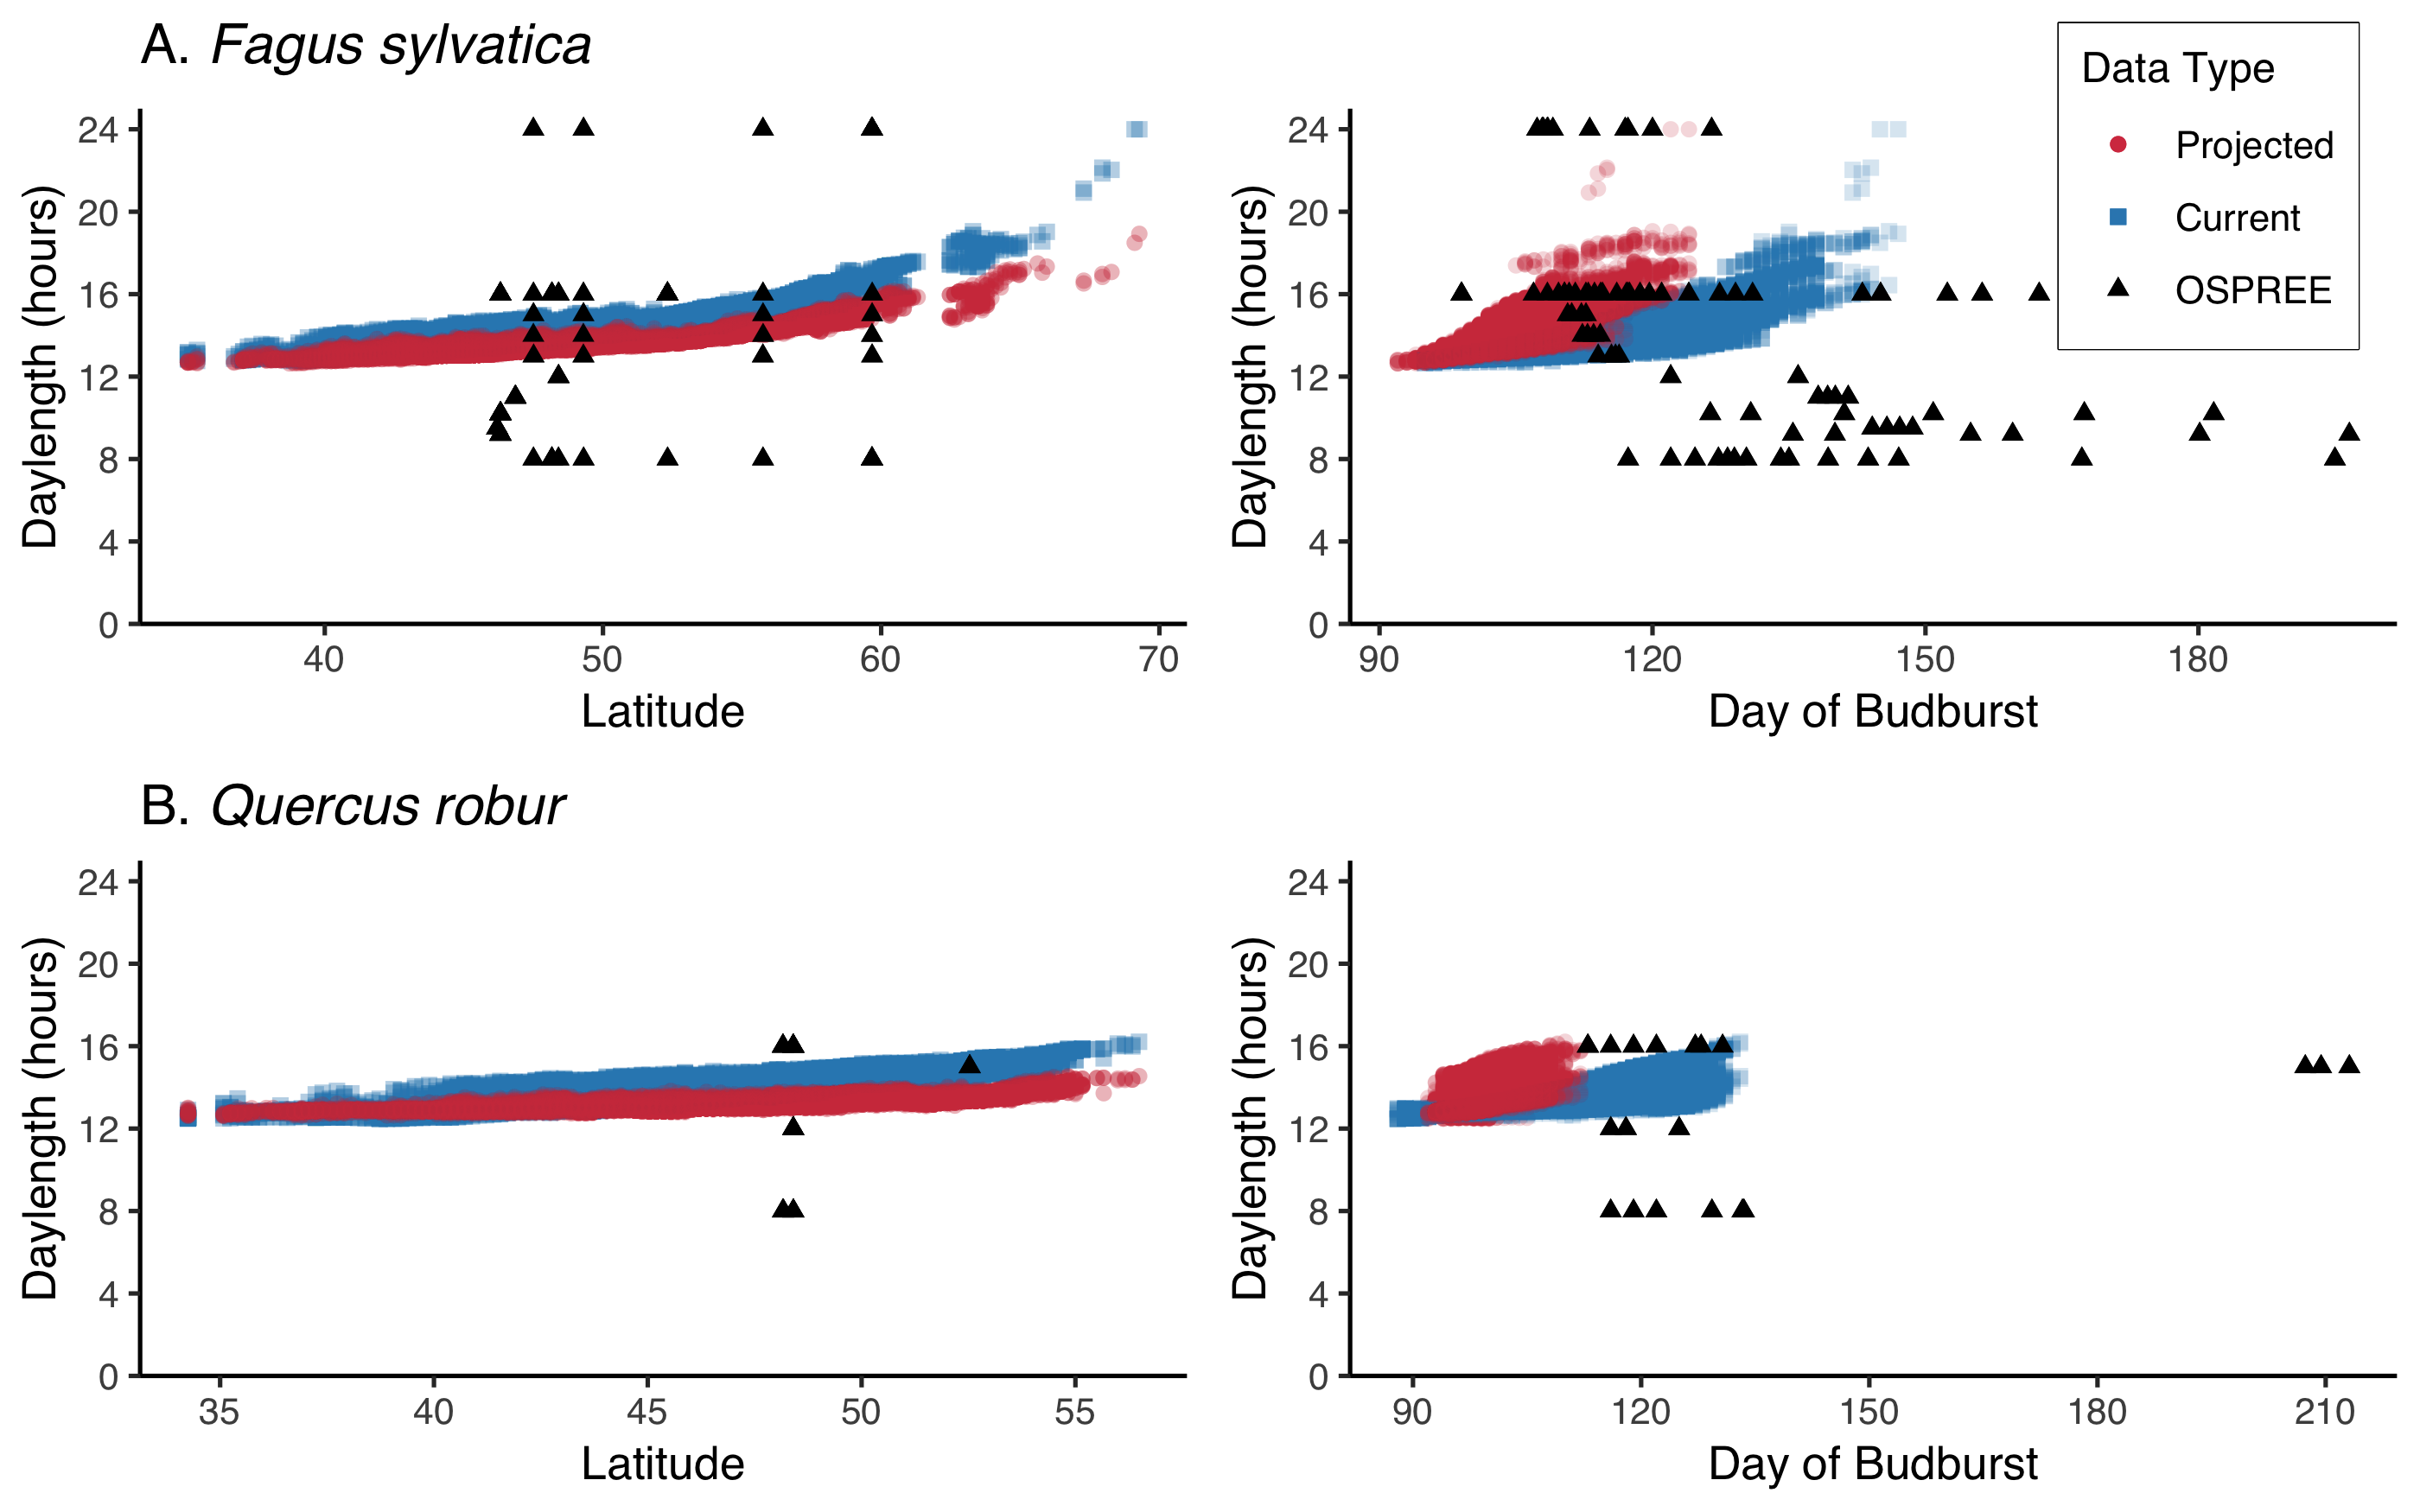
\includegraphics{/Users/aileneettinger/Documents/GitHub/ospree/analyses/photoperiod/figures/2D_actual_combined.png} 
\caption{\textbf{Experimental treatments of daylength as it varies by latitude (left panels) and by day of budburst (right panesl)} for \textit{Fagus sylvatica} (A) and \textit{Quercus robur} (B). For comparison, we show the daylength when budburst occurs in its current and projected ranges. We took current budburst data (1981-2000) and model projections for budburst (2081-2100) using the A1Fi Phenofit scenario \citep{duputie2015} for the two species and compared these points to data obtained from the OSPREE dataset. The OSPREE data points were collected from experiments and days of budburst were calculated from the start of the experiment, rather than from the start of the year. In order to render these points comparable to the current observations and the model projections, we scaled the days to budburst by adding the day of budburst from the first Phenofit observation to all of the OSPREE data points. We only used Phenofit data that had both current and projected data. In panel (B) for \textit{Fagus grandifolia}, we explored the 15 OSPREE data points that have later day to budburst times than the current or projected days to budburst. The majority of those points had 5-8 hours shorter photoperiods than is biologically possible and the last few points had little or no experimental chilling.}%quite longg caption right now- move some to supplemental methods
 \label{fig:fagus}
 \end{figure}
 
\begin{figure}[p]
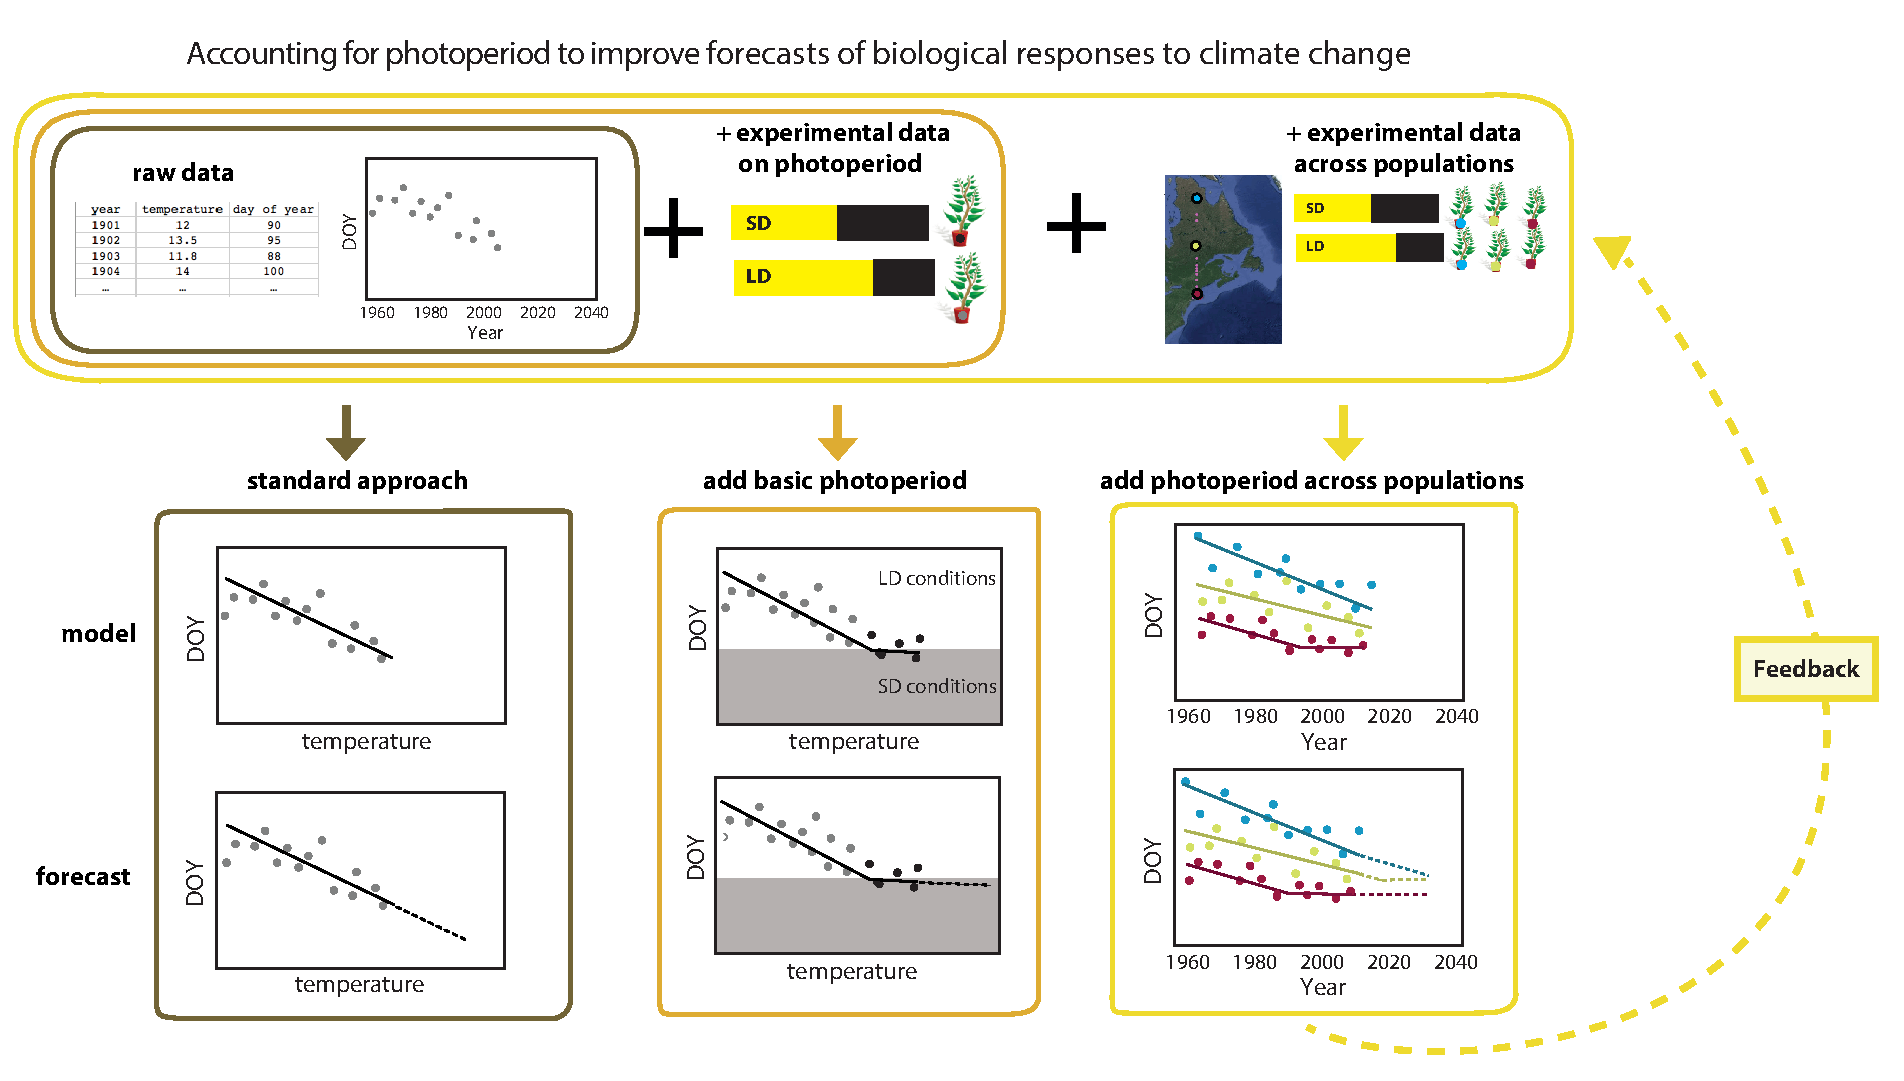
\includegraphics{/Users/aileneettinger/Documents/GitHub/ospree/analyses/photoperiod/figures/photocondiag6.pdf} 
\caption{\textbf{Conceptual diagram of how to include photoperiod in forecasting biological responses to climate change}.}
 \label{fig:condiag}
 \end{figure}
 
%%%%%%%%%%%%%%%%%%%%%%%%%%%%%%%%%%%%%%%%
\end{document}
%%%%%%%%%%%%%%%%%%%%%%%%%%%%%%%%%%%%%%%%
